\documentclass{article}
%% Chapter 1 Section 10: Exponentiation

\usepackage{amsmath}
\usepackage{palatino}
\usepackage{tikz}

\newcommand{\curry}[1]{\emph{curry}(#1)}
\newcommand{\eval}{\emph{eval}}
\newcommand{\id}{\emph{id}}
\begin{document}

\begin{enumerate}
\item [1.10.5.1]
\item [1.10.5.2]
\item [1.10.5.3]
\item [1.10.5.4]
  To show that $\curry{\eval_{AB}} = \id_{(B^A)}$, we fill blanks in the exponent diagram.
  \begin{center}
    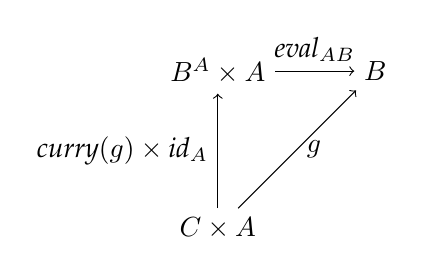
\begin{tikzpicture}
      \node (1) {$B^A \times A$};
      \node [below of=1,yshift=-1cm] (2) {$C \times A$};
      \node [right of=1,xshift=1cm] (3) {$B$};
      
      \draw[->] (2) -- node [right] {$g$} (3);
      \draw[->] (2) -- node [left] {$\curry{g} \times \id_A$} (1);
      \draw[->] (1) -- node [above] {$\eval_{AB}$} (3);
    \end{tikzpicture}
  \end{center}

  In this case, we want to curry the eval function.
  Hence we replace $g$ with $\eval_{AB}$.
  This constricts the domain of $\curry{\eval_{AB}}$ to be $(B^A \times A)$, same as its codomain.
  As $\curry{}$ is unique and shares its domain and codomain with $\id_{B^A}$, it must be the case that $\curry{\eval_{AB}} = id_{B^A}$.
  \begin{center}
    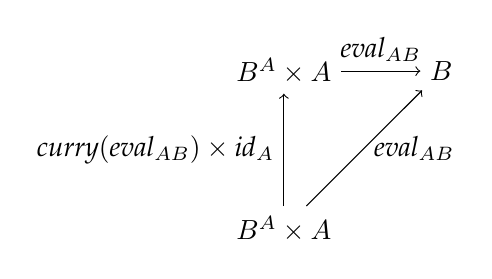
\begin{tikzpicture}
      \node (1) {$B^A \times A$};
      \node [below of=1,yshift=-1cm] (2) {$B^A \times A$};
      \node [right of=1,xshift=1cm] (3) {$B$};
      
      \draw[->] (2) -- node [right] {$\eval_{AB}$} (3);
      \draw[->] (2) -- node [left] {$\curry{\eval_{AB}} \times \id_A$} (1);
      \draw[->] (1) -- node [above] {$\eval_{AB}$} (3);
    \end{tikzpicture}
  \end{center}

\item [1.10.5.5]
\item [1.10.5.6]
\item [1.10.5.7]
\item [1.10.5.8]
\end{enumerate}

\end{document}
